\chapter{KHẢO SÁT NGHIỆP VỤ VÀ ĐẶC TẢ YÊU CẦU HỆ THỐNG}

\section{Khảo sát các bên liên quan và phân tích tác tử người dùng (Actors)}

Khảo sát quy trình vận hành kho thực tế xác định 4 tác tử chính tham gia tương tác với hệ thống:

\begin{table}[h!]
\centering
\caption{Mô tả vai trò và trách nhiệm của các tác tử trong hệ thống}
\begin{tabular}{|l|l|l|}
\hline
\rowcolor{tablehead}
\textbf{Tác tử (Actor)} & \textbf{Mô tả vai trò} & \textbf{Quyền hạn chính} \\ \hline
Quản trị viên (Admin) & Người có toàn quyền quản trị hệ thống và người dùng & Quản lý tài khoản, phân quyền RBAC, cấu hình hệ thống, xem toàn bộ báo cáo và nhật ký kiểm toán \\ \hline
Thủ kho (Warehouse Staff) & Người trực tiếp thực hiện các thao tác xuất nhập tại kho & Lập phiếu nhập kho, lập phiếu xuất kho, quản lý sản phẩm, theo dõi vị trí kệ và kiểm kê tồn \\ \hline
Kế toán kho (Accountant) & Người phụ trách số liệu tài chính và giá trị tồn kho & Xem danh mục, xem lịch sử xuất nhập, kiểm tra định giá tồn kho, xem báo cáo doanh số và phân tích AI \\ \hline
Dịch vụ AI (AI Service) & Tác tử thông minh xử lý ngầm trong hệ thống & Tổng hợp số liệu CSDL, tính tốc độ xuất, dự báo ngày cạn hàng, phát hiện bất thường và trả lời trợ lý \\ \hline
\end{tabular}
\end{table}

\section{Đặc tả các yêu cầu chức năng hệ thống (Functional Requirements)}

Hệ thống được đặc tả thành 10 nhóm yêu cầu chức năng chính, mỗi yêu cầu được gán mã định danh duy nhất để phục vụ công tác truy vết kỹ thuật (Traceability):

\begin{table}[h!]
\centering
\caption{Danh mục đặc tả 10 yêu cầu chức năng chính của hệ thống}
\begin{tabular}{|l|l|l|l|}
\hline
\rowcolor{tablehead}
\textbf{Mã YC} & \textbf{Tên yêu cầu chức năng} & \textbf{Mô tả chi tiết nghiệp vụ} & \textbf{Vai trò áp dụng} \\ \hline
REQ-AUTH & Xác thực \& Phân quyền & Đăng nhập bằng JWT OAuth2 Bearer, mã hóa mật khẩu Argon2, kiểm soát truy cập dựa trên vai trò RBAC & Tất cả \\ \hline
REQ-PROD & Quản lý Danh mục Sản phẩm & Thực hiện CRUD sản phẩm, quản lý mã SKU, phân loại nhóm ngành hàng, đơn vị tính, giá vốn, giá bán, định mức tồn min/max & Admin, Thủ kho \\ \hline
REQ-SUPP & Quản lý Nhà cung cấp & Quản lý thông tin đối tác cung ứng, mã nhà cung cấp, thông tin liên hệ, lịch sử giao dịch cung ứng hàng hóa & Admin, Thủ kho \\ \hline
REQ-LOC & Quản lý Vị trí Lưu trữ & Quản lý danh mục vị trí kệ kho (Khu vực, Kệ, Tầng, Ô) nhằm tối ưu hóa đường đi lấy hàng và lưu kho & Admin, Thủ kho \\ \hline
REQ-IMP & Quản lý Nhập kho & Lập và duyệt phiếu nhập kho từ nhà cung cấp, tự động cập nhật tăng tồn kho và ghi nhật ký biến động kho & Admin, Thủ kho \\ \hline
REQ-EXP & Quản lý Xuất kho Chống âm & Lập phiếu xuất kho cho khách hàng/phòng ban, kiểm tra tồn khả dụng, tự động từ chối và rollback nếu vượt quá tồn kho & Admin, Thủ kho \\ \hline
REQ-AI-ANL & Phân tích Kho AI \& Cảnh báo & Tự động phân tích tốc độ tiêu thụ (Burn-rate), dự báo ngày cạn kho, phát hiện bất thường xuất nhập và gợi ý nhập hàng & Admin, Thủ kho, Kế toán \\ \hline
REQ-AI-NLP & Trợ lý Hỏi đáp Kho NLP & Cung cấp giao diện trò chuyện bằng ngôn ngữ tự nhiên tiếng Việt, trả lời chính xác số lượng tồn và định giá dựa trên CSDL & Admin, Thủ kho, Kế toán \\ \hline
REQ-DASH & Bảng điều khiển KPI & Trực quan hóa thời gian thực các chỉ số: tổng SKU, tổng số lượng tồn, tổng định giá tồn kho, số mã dưới định mức, biểu đồ xuất nhập 30 ngày & Tất cả \\ \hline
REQ-AUDIT & Nhật ký Kiểm toán Biến động & Ghi vết đầy đủ mọi biến động tăng giảm kho (Mã hàng, số lượng trước, số lượng sau, loại phiếu, người thực hiện, thời gian) & Admin, Kế toán \\ \hline
\end{tabular}
\end{table}

\section{Đặc tả các yêu cầu phi chức năng (Non-Functional Requirements)}

Hệ thống đáp ứng các tiêu chuẩn chất lượng công nghiệp thông qua các yêu cầu phi chức năng sau:

- NFR-SEC (Bảo mật): Sử dụng chuẩn JWT với thời gian hết hạn hợp lệ; mật khẩu lưu trữ trong CSDL được băm bằng thuật toán Argon2; bảo vệ các API nhạy cảm bằng RBAC Middleware.

- NFR-PERF (Hiệu năng): Thời gian đáp ứng của các API truy vấn nghiệp vụ thông thường nhỏ hơn 100ms; thời gian phản hồi của dịch vụ phân tích AI nhỏ hơn 1.5 giây.

- NFR-REL (Độ tin cậy): Hệ thống đảm bảo tính toàn vẹn dữ liệu kế toán thông qua giao dịch ACID; tuyệt đối không để xảy ra hiện tượng tồn kho âm (Negative Inventory).

- NFR-DATA (Toàn vẹn CSDL): CSDL được chuẩn hóa ở dạng chuẩn 3NF, loại bỏ dư thừa dữ liệu và đảm bảo tính nhất quán qua các khóa ngoại (Foreign Keys).

\section{Mô hình hóa chức năng bằng sơ đồ Use Case tổng thể}

Sơ đồ Use Case tổng thể mô hình hóa toàn bộ mối quan hệ tương tác giữa 4 tác tử và các phân hệ chức năng trong hệ thống quản lý kho tích hợp AI:

\begin{figure}[h!]
\centering
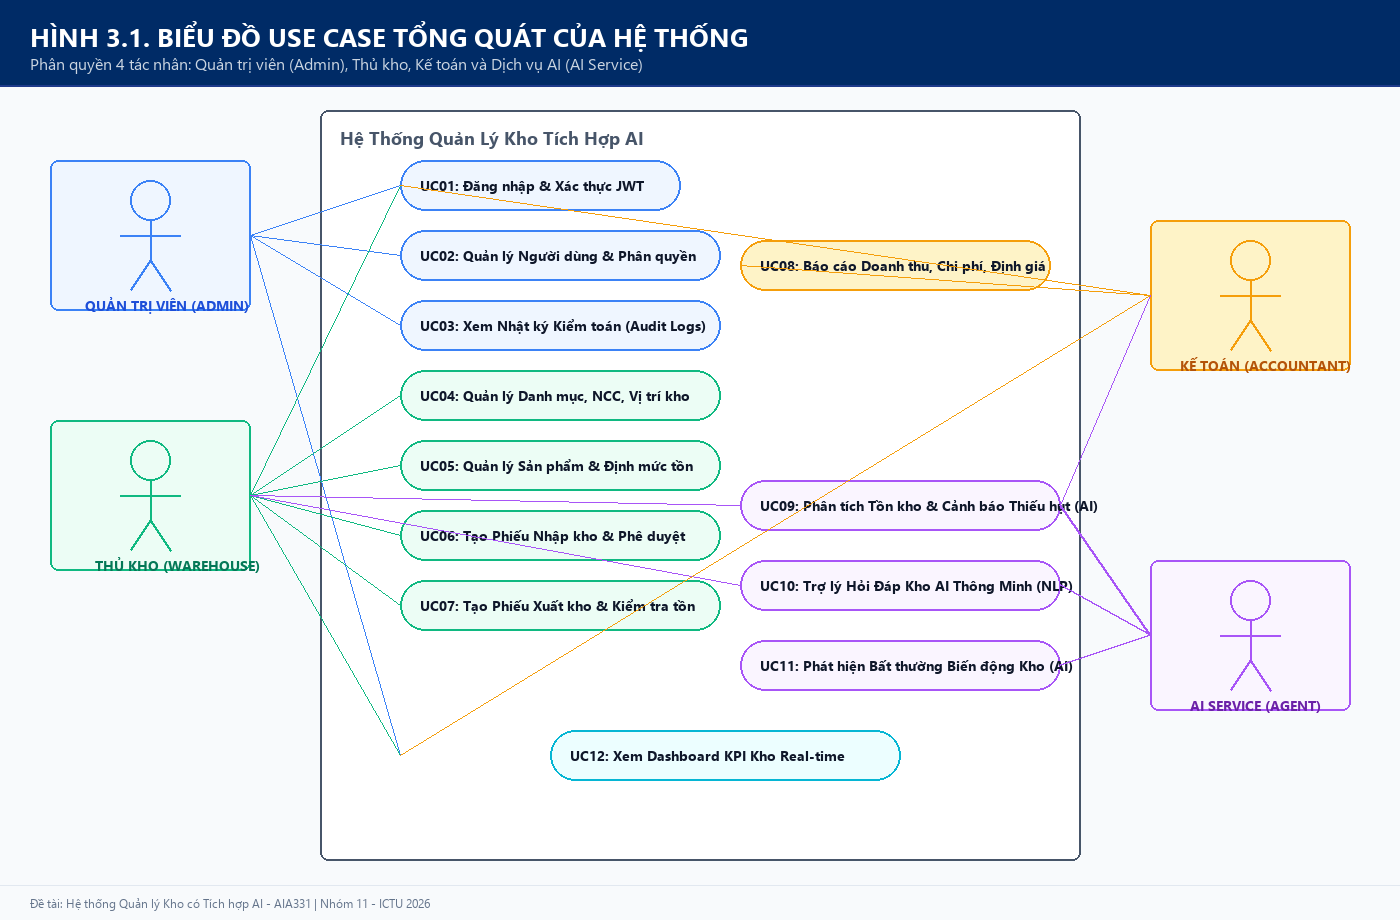
\includegraphics[width=0.92\textwidth]{figures/usecase.png}
\caption{Sơ đồ Use Case tổng thể hệ thống quản lý kho tích hợp AI}
\end{figure}

